Il gruppo \Gruppo{} punta a sviluppare un piano di lavoro che sia conforme al modello incrementale sebbene la mancanza di esperienza possa essere un fattore limitante nella corretta applicazione dei principi previsti da tale modello.

\subsection{Descrizione}
La scelta di un modello di sviluppo porta dei vincoli sulla pianificazione e sulla gestione del progetto.
Il gruppo vorrebbe raggiungere un modello di sviluppo di tipo incrementale per il \glo{ciclo di vita} del software per i seguenti motivi:
\begin{itemize}
    \item può produrre valore ad ogni incremento, aiutando a fissare meglio i requisiti per gli incrementi
    successivi;
    \item ogni incremento riduce il rischio di fallimento;
    \item le funzionalità principali e/o critiche sono sviluppate nei primi incrementi che diventano via via più stabili.
\end{itemize}





Nel modello incrementale i requisiti vengono classificati in base alla loro importanza strategica. In
questo modo quelli più importanti vengono trattati prima. Questo ne aumenta la chiarezza e la
facilità di soddisfazione. I requisiti meno importanti invece vengono soddisfatti dopo quelli principali, venendo cosi inseriti in un sistema già stabilizzato.
Il metodo di lavoro sarà quindi questo:
\begin{itemize}
    \item in ogni fase di lavoro vengono prefissati degli incrementi che devono essere prodotti entro una data di
    scadenza decisa dal gruppo;
    \item il lavoro viene diviso tra i membri del gruppo;
    \item al termine del periodo prefissato i membri del gruppo si riuniranno per analizzare il lavoro svolto da ogni
    componente, segnalando eventuali problemi o difficoltà;
    \item sarà compito dei verificatori controllare il lavoro svolto dagli altri membri del gruppo e sollevare
    eventuali incongruenze o errori;
    \item alla fine di questa \glo{verifica} seguirà una nuova discussione di gruppo per stabilire se gli obiettivi
    dell’incremento sono stati soddisfatti.
\end{itemize}






\begin{figure}[h!]
    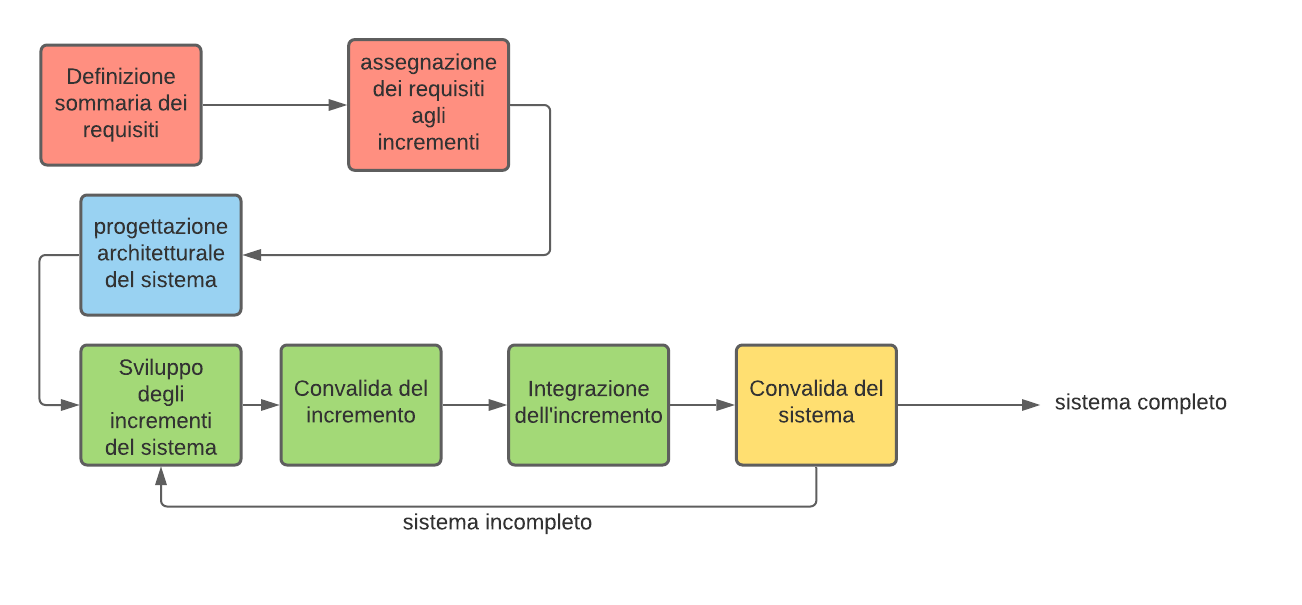
\includegraphics[width=1\textwidth]{./src/ModelloSviluppo/src/img/diagramma modello di sviluppo.png}
    \caption{Modello Incrementale tratto dal libro di Ian Somerville:Software Engineering ottava edizione}
\end{figure}